\documentclass[12pt]{report}
\usepackage[margin=1.2in]{geometry}
\usepackage{fancyhdr}
\usepackage{framed, color}
\usepackage{graphicx}
\usepackage{url}
\usepackage{mathtools}  
\usepackage{amsmath}
\usepackage{amssymb}
\usepackage{tabulary}
\usepackage{booktabs}
\usepackage{hyperref}
\usepackage{float}
\usepackage{natbib}

\hypersetup{
    colorlinks,
    citecolor=black,
    filecolor=black,
    linkcolor=blue,
    urlcolor=black
}

\newcommand\frontmatter{%
  \cleardoublepage
  %\@mainmatterfalse
  \pagenumbering{roman}}

\newcommand\mainmatter{%
  \cleardoublepage
 % \@mainmattertrue
  \pagenumbering{arabic}}

\newcommand\backmatter{%
  \if@openright
    \cleardoublepage
  \else
    \clearpage
  \fi
 % \@mainmatterfalse
}



\title{\textbf{Application of Probabilistic PCA}}
\author{
		\bf{RnD Project Report}\\
        \\
        \emph{Submitted in partial fulfillment of requirements for the degree of}\\
        \bf{Bachelor of Technology (Honors)}\\
        \\
        \emph{by}\\
		\bf{Aditya Kumar Akash}\\
        \bf{Roll No : 120050046}\\
        \\
        \emph{under the guidance of}\\
		\bf{Prof. Suyash Awate}\\
        \\\\
        
\includegraphics[height=3.5cm]{./iitb_logo.jpg}\\
        \\
		\bf{Department of Computer Science and Engineering}\\
        \bf{Indian Institute of Technology Bombay}\\
        \bf{Mumbai 400076, India}\\
}
\date{April, 2016}

\bibliographystyle{plain}

\begin{document}
\frontmatter
\maketitle
\pagebreak
\tableofcontents
\pagebreak

\chapter*{\center{Abstract}}
Principal Component analysis (PCA) is a classical data analysis technique that finds linear transformations of data that retain the maximal amount of variance. The classical version is not based on a probability model. Researchers have proposed a probabilistic model of PCA which is closely related to factor analysis. In this work, we understand the Probabilistic PCA (PPCA) and analyse how it handles missing data situations in which we cannot apply standard PCA. We also try to obtain a comparision in performance of PPCA with a variant of PCA.

\pagebreak

\chapter*{\center{Acknowledgements}}
I am sincerely indebted to my advisor, Prof. Suyash Awate, IIT Bombay, for his constant support and guidance throughout the course of this project. His experience and insight in the fields of machine learning, image processing and varied aspects of computer science in general, was valuable in boosting my interest on this topic. \\\\
I finally and especially would like to thank my parents and my whole family for their support and trust in all of my endeavours. The morals they have imparted stayed and would stay close to me always. I also thank my friends for giving a helping hand during hard times.
\pagebreak


\mainmatter
\chapter{Introduction}

Principal Component analysis (PCA) is a ubiquitous tool for dimensionality reduction.  It has many applications data compression, visualization, image processing, exploratory data analysis, pattern recognition and time series prediction. \\
There are a number of optimization criteria to derive PCA. The most important of these is in terms of stardardized linear projection which maximizes the variance in the projected space \cite{PCA}. Assume that $\{y_i\}, i \in \{1, 2, ..., n\}$ is a set of $d$ dimensional data vectors. Then the $k$ principal axes $\{w_j\}, j \in \{1, 2, ..., k\}$ are those orthogonal axes onto which the retained variance under projection is maximal. It can be shown that $w_j$ are given by $k$ dominant eigen vectors (those with largest eigen values, $\lambda_j$) of the sample covariance matrix  
\begin{center}
\begin{equation}
	\mathbf{S = \sum_{i=1}^n (y_i - \bar{y})(y_i - \bar{y})^T}
\end{equation}
\end{center}
where $\mathbf{\bar{y}}$ is the sample mean, such that
\begin{equation}
\mathbf{Sw_j=\lambda_jw_j}
\end{equation}
The $k$ principal components of the observed vector $\mathbf{y_i}$ are given by the vector 
\begin{equation}
\mathbf{x_i=W^T(y_i - \bar{y})}
\end{equation}
where $\mathbf{W = (w_1;w_2;...;w_k)}$. The variables $\mathbf{x_i}$ are uncorrelated such that the covariance matrix $\sum_{i=1}^n\frac{\mathbf{x_ix_i^T}}{n}$ is diagonal with elements $lambda_i$.\\
A complementary property of PCA is that of all the orthogonal linear projections, the principal component minimizes the squared reconstruction error. However, PCA does not provide a probabilistic model of data. This gives motivation for PPCA.

\section{Motivation}
A probabilistic formulation of PCA from a Gaussian latent variable model is obtained. This is closely related to factor analysis. PCA could be viewed a limiting case of such a Gaussian model. In such a formulation, the principal axes emerge as maximum likelihood parameter estimates. Such a probabilistic formulation is intuitively applealing, as the definition of a likelihood measure enables comparison with other probabilistic techniques, while facilitating statistical testing and permitting the application of Bayesian methods. Further motivation behind a probabilistic PCA is that it conveys additional practical advantage as :
\begin{itemize}
\item The probability model offers the potential to extend the scope of conventional PCA, such as using probabilistic mixtures and PCA projections in missing data case.
\item PPCA can be utilized as a general Gaussian density model. This allows the maximum likelihood estimates for the parameters associated with the covariance matrix to be efficiently computed from the data principal components.
\end{itemize}


\chapter{Background}

As we have seen, Program Synthesis is the task of discovering an executable piece of code from user intent given a high level specification of the goal. As we shall see later, this high level specification can take different forms and in fact this becomes a dimension \cite{gulwani2010dimensions} along which program synthesis can be classified. For now, let us understand program synthesis through an example.

\section{An Example of Program Synthesis}
Below is a toy example \footnote{adopted from \url{https://en.wikipedia.org/wiki/Program_synthesis}}, of derivation of a functional program to compute the maximum M of two numbers x and y. \\

\begin{table}[h!]
\centering
\label{max_synthesis_axioms}
\begin{tabular}{|l|l|l|}
\hline
No. & Assertions     			& Origin 		\\ \hline
1   & $A = A$        			& Axiom     	\\
2   & $A \leq A$				& Axiom     	\\
3   & $A \leq B \vee B \leq A$ 	& Axiom     	\\ \hline
\end{tabular}
\caption{Some basic axioms related to comparison}
\end{table}

\noindent
To begin with, we consider the assertions mentioned in table 2.1 as our axioms. As you can see, these axioms are very basic and just state the laws of trichotomy. However, we make use of these to derive a functional program that computes the maximum of two numbers; something that is non-trivial to obtain from just these axioms (at least for a computer). \\

\begin{table}[h!]
\centering
\label{max_synthesis}
\begin{adjustwidth}{-0.6cm}{}
\begin{tabular}{|l|l|l|l|}
\hline
No. & Goal & Program & Origin \\ \hline
10  & $x \leq M \wedge y \leq M \wedge (x = M \vee y = M)$ & $M$ & Specification\\
11  & $(x \leq M \wedge y \leq M \wedge x = M) \vee (x \leq M \wedge y \leq M \wedge y = M)$ &    $M$     		& Distr(10)  	\\
12  & $x \leq M \wedge y \leq M \wedge x = M$ & $M$ & Split(11) \\
13  & $x \leq M \wedge y \leq M \wedge y = M$ & $M$ & Split(11) \\
14  & $x \leq x \wedge y \leq x$ & $x$ & Resolve(12,1) \\
15  & $y \leq x$ & $x$ & Resolve(14,2) \\
16  & $\neg (x \leq y)$ & $x$ & Resolve(15,3) \\
17  & $x \leq y \wedge y \leq y$ & $y$ & Resolve(13,1) \\
18  & $x \leq y$ & $y$ & Resolve(17,2) \\
19  & $true$ & $x \leq y ? y : x$ & Resolve(18,16) \\ \hline
\end{tabular}
\end{adjustwidth}
\caption{Example synthesis of maximum function using the axioms in table 2.1}
\end{table}

\noindent
Starting from the requirement description ``The maximum is larger than any given number, and is one of the given numbers'', the first-order formula $\forall X \forall Y \exists M : X \leq M \wedge Y \leq M \wedge (X = M \vee Y = M)$ is obtained as its formal translation. This formula is to be proved. By reverse Skolemization, the specification in line 10 (in table 2.2) is obtained, an upper- and lower-case letter denoting a variable and a Skolem constant, respectively. After applying the distributive law in line 11, the proof goal is a disjunction, and hence can be split into two cases, viz. lines 12 and 13. Turning to the first case, resolving line 12 with the axiom in line 1 leads to instantiation of the program variable M in line 14. Intuitively, the last conjunct of line 12 prescribes the value that M must take in this case. Formally, this conjunct unifies syntactically with the axiom on line 1 by substituting $x$ for $M$ as well as $A$. On making this substitution throughout our goal in line 12, we reach the goal in line 14, the first conjunct of which is trivially true through the axiom in line 2. Thus for the case of $\neg (x \leq y)$, we obtained the program to be $x$. A similar reasoning for the goal in line 13 leads us to the program $y$ for the case of $x \leq y$. We combine both these goals to obtain a goal in line 19 which is $true$ always. The program corresponding to this line is the one we aimed to compute.

\section {A Different Example of Program Synthesis}
In the above example, we have seen the computation of a program starting from a specification that is essentially a logical representation of our goal. It relates logically, the input and output of our program. Though logical representations present a succinct way to provide a formal specification of our desired program, they are often difficult to obtain and use in practice. On the contrary, having an inefficient program to begin with, is often quite useful as we have a correct and working program at the very start. This can continuously be written into a more and more efficient program through calculation rules, such that the correctness in preserved at each step. Both these methods of problem specification are only different ways of conveying user intent. We discuss this in detail in the next section. \\\\
Let us now look at the following example of program derivation, where we want to obtain a program for calculating the minimum element among a list of integers. Consider the following functional specification for doing the same. \\\\

\begin{align*}
minimum &=\: head\: \circ\: sort \\
sort [] &=\: [] \\
sort (x : xs) &=\: insert\: x\: (sort\: xs) \\
insert\: a\: [] &=\: [a] \\
insert\: a\: xs &=\: if\: (a\: <\: head\: xs)\: then\: (a\: :\: xs)\: else\: (head\: xs)\: :\: (insert\: a\: (tail\: xs)) \\
head\: (x\: :\: xs) &=\: x
\end{align*}

\noindent
We derive a recursive definition of minimum from the above specification, by inducting on the input list.

\vspace{0.5em}
\begin{equation*}
\begin{split}
minimum\: [x] &= head(sort\: [x]) \\\\
&= \{\bf{unfolding}\: sort\} \\ &\quad \; head\: (insert\: x\: (sort\: [])) \\\\
&= \{\bf{definition\: of}\: sort\} \\ &\quad \; head\: (insert\: x\: []) \\\\
&= \{\bf{definition\: of}\: insert\} \\ &\quad \; head\: [x] \\\\
&= \{\bf{definition\: of}\: head\} \\ &\quad \; x
\end{split}
\end{equation*}

\vspace{1em}
\begin{align*}
minimum\: (x\: :\: xs)
            &= head\: (sort\: (x\: :\: xs)) \\\\
 			&= \{\bf{unfolding}\: sort\} \\
 			   &\quad \; head\: (insert\: x\: (sort\: xs)) \\\\
 			&= \{\bf{unfolding}\: insert\} \\
 			   &\quad \; head\: (if\: (x < head\: (sort\: xs))\: then\: x\: :\: (sort\: xs) \\
 			   &\quad \quad \quad \quad else\: (head\: (sort\: xs))\: :\: (insert\: x\: (tail\: (sort\: xs))) \\\\
 			&= \{\bf{if\: promotion\: rule}\: :\: f(if\: e_1\: then\: e_2\: else\: e_3)\: =\\
 			   &\qquad \qquad \qquad \bf{if}\: e_1\: then\: (f\: e_2)\: else\: (f\: e_3)\} \\
 			   &\quad \; if\: (x < head(sort\: xs))\: then\: head(x\: :\: (sort\: xs)) \\
 			   &\quad \; else\: head\: (head\: (sort\: xs)\: :\: insert\: x\: (tail\: (sort\: xs))) \\\\
 			&= \{\bf{definition\: of\: head}\} \\
 			   &\quad \; if\: (x < head(sort\: xs))\: then\: x\: else\: head(sort\: xs) \\\\
 			&= \{\bf{abstracting\: out\: head(sort\: xs)\: and\: folding\: back\: minimum}\} \\
 			   &\quad \; if\: (x < y)\: then\: x\: else\: y\\
 			   &\quad \quad \quad where\: y = minimum\: xs
\end{align*}

\section{Dimensions of Program Synthesis}
We know that compilers and assemblers mostly translate a program written in a structured high-level language into a low-level or machine language in a syntax-directed fashion. While on the other hand, program synthesizers take as input the user intent through a variety of constraints such as logical relations between inputs and outputs, partial or inefficient programs, natural language, input-output examples, etc. Then they process these constraints and come up with an output program after searching through a space of programs. In this section, we briefly describe the dimensions along which program synthesizers may be classified, partly in accordance to Sumit Gulwani \cite{gulwani2010dimensions}, excerpts from which have been adopted here.

\subsection{Input Specification}
One of the most important aspects of program synthesis from the user's perspective is the mechanism to specify his intent. As we see below, some of the main choices possible for this are logical specifications, natural language specifications, input-output examples and higher-order, inefficient or partial programs. Depending on the user's skill and the task underlying, a particular choice of the specification may be more suited.

\subsubsection{Logical Specifications}
A  logical  specification is a logical relation between inputs and outputs of a program. It can act as a precise and succinct form of functional specification of the desired program. For example, the logical specification for a program that finds out the maximum of two numbers $x$ and $y$ as $M$ is as follows (recall from the example in section 2.1): \\\\
$x \leq M \wedge y \leq M \wedge (x = M \vee y = M)$ \\\\
Clearly the above logical expression relates the inputs and the output and has to hold for any program that computes the maximum correctly. It merely states that the maximum must be greater than or equal to both the numbers and should be equal to one of them. As you can see, this is only a specification of our end goal and it says nothing about how we arrive at a program which satisfies it. \\\\
As another example, consider any sorting algorithm for a list of numbers. The logical specification for the sorted list $S$ of a given list $L$ of size $n$ would assert that $S$ is a \emph{permutation} of the list $L$ and has its elements \emph{sorted}. \\\\
Though synthesis systems that accept user intent in the form of logical specifications exist, compared to other forms of specifications such as input-output examples and partial/inefficient programs, logical relations require additional knowledge of logic. Further they might be harder to get right, and may not be a preferred form of specification for end-users.

\subsubsection{Input-Output Examples}
In several scenarios, input-output examples can act as the simplest form of specification, with relatively little chances of error. Quite contrary to what it may seem initially, input-output examples, in conjunction with interactive rounds, can often play the role of a full functional specification. \\\\
It is natural to ask what prevents the synthesizer from synthesizing a trivial program that simply performs a table lookup as follows, when provided with the set $\{(x_1,y_1), (x_2,y_2),..., (x_n,y_n)\}$ of input-output pairs. \\
\begin{lstlisting}
switch x
	case x_1: return y_1;
	case x_2: return y_2;
		.
		.
		.
	case x_n: return y_n;
\end{lstlisting}
We can defend ourselves from obtaining such trivial solutions by restricting the search space of our function. In particular, we could allow only for a bounded number of statements or conditionals. Another concern with input-output examples is the selection criterion and the number of input-output examples. In other words, identifying what constitutes a good input-output example, and how many examples should the user provide? The user may start by providing few input-output examples (possibly a couple of examples for each of the corner cases) and then add more input-output examples in each interactive round. The interaction may either be driven by the user or by the synthesizer, briefly described below. \\\\
\textbf{User Driven Interaction} The user inspects the program returned by the synthesizer, studies/tests it to find any discrepancy in the behaviour of the program and the expected behaviour on a new input. If so, the user repeats the synthesis process after adding the new input-output pair to the list of input-output examples. \\\\
\textbf{Synthesizer Driven Interaction} Given a set of input-output pairs, the synthesizer searches for programs that map each input in the given set to the corresponding output. Assuming that the search space is restricted, there would only be a few satisfying programs. If the synthesizer finds at least two satisfying programs $P_1$ and $P_2$, it declares the user specification to be partial. In such a case, it generates a \emph{distinguishing input}, on which both programs generate different outputs, and presents it to the user asking for its corresponding output. The synthesis process is then repeated with this input-output pair added to the previous examples.\\\\
This type of synthesis, where search for programs is driven by input-output examples is known as \emph{Inductive Synthesis}. This is the subject of Emmanuel Kitzelmann's thesis \cite{kitzelmann2011combined}, where he describes an algorithm \emph{Igor2} that combines analytical and search-based approaches for inductive synthesis. We discuss about it briefly in chapter 5.

\subsubsection{Programs}
Programmers might sometimes find a programming language as the best means of specifying their intent. Even for applications such as discovery of new algorithms, some people might find it easier to write the specification as an inefficient program rather than a logical relation. We have seen an example of this in section 2.2, where our initial function for finding the minimum of a list of numbers merely picked the head of the list after sorting. Clearly the sorting function used there would take time $O(n^2)$ where $n$ is the size of the input list. This is also the time complexity for the initial algorithm. However, through equational rewriting and unfolding, we derive an efficient program that takes only $O(n)$ time.

\subsubsection{Natural Language}
Given advances in natural language processing, it is possible to map
natural language sentences into logical representations \cite{zettlemoyer2009learning}. Natural language can be used as a substitute for logical relations, and end-users might find it very valuable. In particular, natural language interfaces have been designed to query databases to accommodate the need of end-users who interact with databases, but are intimated by the idea of using languages such as SQL. Infact, I myself have worked before on such a project for translating queries from english to SQL given the underlying database schema. There I tried to perform this translation through a deterministic method involving \emph{Context Free Grammars} (CFGs) as well as statistically through a \emph{Machine Translation} system called \emph{Moses}. Here is a link to the project repository \url{https://github.com/shyamjvs/cs626_project}. \\\\
However, the disadvantage with natural language is that it can be ambiguous. More over, from the point of program synthesis, we are not very much interested in this form of user intent as eventually natural language must be converted to a structured (possibly logical) representation for a machine to work with. Thus we choose to neglect natural language inputs, thinking of them as more of the \emph{Machine Translator}'s and \emph{Natural Language Processor}'s job rather than the \emph{Program Synthesizer}'s job.

\subsection{Search Space}
The second dimension in program synthesis is the space of programs over which the desired program will be searched. This choice is made by the developer of the synthesizer and may optionally be restricted by the user of the synthesizer. \\\\
The developer of the synthesizer needs to strike a good balance between expressiveness and efficiency of the search space. On one hand, the space of the programs should be large/expressive enough to include programs that users care about. While on the other hand, the space of the programs should be restrictive enough so that it is amenable to efficient search, and it should be over a domain of programs that are amenable to efficient reasoning. \\\\
The user of the synthesizer can optionally restrict the search space to obtain programs with specific resource usage. For example, the user might desire a loop-free program, or a program whose memory usage does not exceed a specified amount. \\\\
Broadly speaking, the search space can be over the space of (Turing-complete) programs, or restricted form of computational models such as grammars and logics. For the purpose of our work, we choose to neglect computational models involving learning of grammars and logics. The key choice we decide to make is among \emph{Functional} and \emph{Imperative} programs, as these are most widely in use at present. \\\\
We choose functional programming over imperative programming due to better suitability to program synthesis and verification. The most significant differences between both stem from the fact that functional programming avoids side effects, which are used in imperative programming to implement state and I/O. Pure functional programming completely avoids side-effects and provides \emph{Referential Transparency}, which makes it easier to verify, optimize, and parallelize programs, and easier to write automated tools to perform those tasks. \\\\
Further, higher-order functions are rarely used in traditional imperative programming. Where an imperative program might use a loop to traverse a list, a functional program would use a different technique. It would use a higher-order function that takes as arguments a function and a list. The higher-order function would then apply the given function to each element of the given list and then return a new list with the results. This again is amenable to program verification, as iteration would involve state maintenance. So we achieve recursion (thus iteration) in functional programming, without losing referential transparency.
\chapter{Probabilistic PCA}
\section{The Probability model}
The model bears similarity to the factor analysis model, 
\begin{equation}
\mathbf{y = Wx + \mu + \epsilon}
\end{equation}
with the assumption of isotropic gaussian noise model $\mathcal{N}(0, \sigma^2\mathbf{I})$. This gives as $x$-conditional distribution over $y$-space as
\begin{equation}
\mathbf{t|x \sim \mathcal{N}(Wx + \mu, \sigma^2I)}
\end{equation}
With $x \sim \mathcal{N}(0, \mathbf{I})$, the marginal distribution for $y$ is given by 
\begin{equation}
\mathbf{t \sim \mathcal{N}(\mu, C)}
\end{equation}
where oberservation covariance model is specified by $\mathbf{C = WW^T + \sigma^2I}$. \\
The log-likelihood is then 
\begin{equation}
\mathcal{L} = -\frac{N}{2}{d \text{ln}(2\pi) + \text{ln}|\mathbf{C}| + \text{tr}(\mathbf{C^{-1}S})}
\end{equation}
where 
\begin{equation}
	\mathbf{S} = \frac{1}{N}\sum_{i=1}^N\mathbf{(y_i - \mu)(y_i - \mu)^T}
\end{equation}
The maximum-likelihood estimates for $\mu$ is given by the mean of the data, in which ase $\mathbf{S}$ is the sample covariance. Estimates of $\mathbf{W}$ and $\sigma^2$ is obtained by $EM$ algorithm.
\pagebreak
\section{EM method for PPCA}
In the $EM$ approach to maximize likelihood for PPCA, we consider latent variables $\mathbf{x_i}$ to be 'missing' data and the 'complete' data to comprise the observations together with latent variables. Corresponding complete log-likelihood is then :
\begin{equation} \label{eq1}
\mathcal{L_C} = \sum_{i=1}^N\text{ln}\{p(\mathbf{y_i, x_i})\}
\end{equation},
where, in PPCA, we get
\begin{equation}
p(\mathbf{y_i, x_i}) = (2\pi \sigma^2)^{-d/2}\text{exp}\big\{-\frac{||\mathbf{y_i - Wx_i - \mu}||}{2\sigma^2}\big\}(2\pi)^{-k/2}\text{exp}\big\{-\frac{||\mathbf{x_i}||}{2}\big\}
\end{equation}
The posterior is given by 
\begin{equation}
\mathbf{x|y} \sim \mathcal{N}(\mathbf{M^{-1}W^T(y-\mu), \sigma^2M{-1}})
\end{equation}
where $\mathbf{M} = W^TW + \sigma^2I$.
From the appendix B of \cite{PPCA} we obtain following \\\\
\textbf{E-Step} : 
\begin{equation}
\mathbf{\langle x_i\rangle = M^{-1}W^T(y_i - \mu)}
\end{equation}
\begin{equation}
\mathbf{\langle x_ix_i^T\rangle = \sigma^2M^{-1} + \langle x_i\rangle \langle x_i\rangle^T}
\end{equation}
\textbf{M-Step} :
\begin{equation}
\mathbf{\tilde{W} = \big[ \sum_i(y_i-\mu)\langle x_i\rangle \big]\big[\sum_i\langle x_ix_i^T\rangle \big]^{-1}}
\end{equation}
\begin{equation}
\mathbf{\sigma^2 = \frac{1}{Nd}\sum_i\big\{ ||y_i-\mu||^2 - 2\langle x_i\rangle^T\tilde{W}^T(y_i-\mu) + \text{tr}(\langle x_ix_i^T\rangle\tilde{W}^T\tilde{W}) \big\}}
\end{equation}

The paper \cite{PPCA} shows the combination of both of the above steps rewritten as 
\begin{equation}
\mathbf{\tilde{W} = SW(\sigma^2I + M^{-1}W^TSW)^{-1}}
\end{equation}
\begin{equation}
\mathbf{\sigma^2 = \text{tr}(S-SWM^{-1}\tilde{W}^T)}
\end{equation}
$\mathbf{S}$ is the sample covariance.\\
Analysis of thes equations show that in normal PCA calculation we require calculation of $\mathbf{S}$ which takes $\mathcal{O(N}d^2)$ operations. But in case of above EM formulation, we only need to compute $\mathbf{SW}$ as $\mathbf{\sum_i x_i(x_i^TW)}$ which takes $\mathcal{O(N}dk)$ operations. Thus when $k\ll d$, considerable computational savings would be obtained. This is one of the benefits of using the EM version of PPCA.

\section{Properties of MLEs}
In paper \cite{PPCA} it is shown that with $\mathbf{C = WW^T + \sigma^2I}$, likelihood \ref{eq1} is maximized when 
\begin{equation}
\mathbf{W_{ML} = U_k(\Lambda_k - \sigma^2I)^{1/2}R}
\end{equation}
where $k$ column vectors in $\mathbf{U_k}$ are the principal eigenvectors of $\mathbf{S}$, with corresponding eigenvalues in $\Lambda_k$, and $\mathbf{R}$ is arbitary orthogonal rotation matrix. \\
When $\mathbf{W = W_{ML}}$, MLE for $\sigma^2$ is
\begin{equation}
\sigma^2_{ML} = \frac{1}{d - k}\sum_{j=k+1}^d\lambda_j
\end{equation}
which has \textbf{interpretation of variance lost in projection, averaged over the lost dimension}. Using this we can see how this lost variance is subtracted from the eigen vectors in the estimation of $\mathbf{W_{ML}}$.
\chapter{Missing Data}
\section{PPCA with Missing Data}
One of the motivation of using PPCA is that it provides interpretation to the data that is missing from the observation variable. Such \emph{missing data variables are assumed to be 'parameters' in the model} and a generic EM algorithm is designed to handle the case.\\
An example of missing data case would be in computer vision field, when we model a dodecahedran from a sequence of segmented images. One sample of data would contain only information (in form of normals) for only 6 of the faces, while rest is missing data.\\\\
In these cases the \textbf{E-step} of EM algorithm is generalized to following :\\
\textbf{Generalized E-step} \citep{SPCA} 
\begin{itemize}
\item If $\mathbf{y}$ is incomplete, then we find a unique pair of points $\mathbf{x^*, y^*}$ (such that $\mathbf{x^*}$ lies in the current principal subspace and $\mathbf{y^*}$ lies in the subspace defined by the known information about $\mathbf{y}$) which minimize the norm $||\mathbf{Wx^*-y^*+\mu}||^2$. Now we set the corresponding expectation of $\mathbf{x}$ to $\mathbf{x^*}$ and correspoinding observed variable $\mathbf{y}$ to $\mathbf{y^*}$. The solution is obtained by finding solution to a particular constrained matrix.
\item If $\mathbf{y}$ is complete, then $\langle \mathbf{x} \rangle$ is found as before.
\end{itemize}
The above steps emerge as a result of treating the missing values as parameters to the model. The optimization problem results from maximizing the likelihood of the complete data. 
\pagebreak
\section{PCA with Missing Data}
In this work we also try to compare following PCA modification for missing data. 
\begin{itemize}
\item \textbf{PCA with reference to Factor analysis} : In this approach we try to estimate the missing values using the minimization of $||\mathbf{Wx^*-y^*+\mu}||^2$. $\mathbf{x}$ is the latent variable. In each iteration, first $\mathbf{y}$ is estimated using this minimization, then $\mathbf{W}$ is estimated by finding $k$ principal component of covariance of $\mathbf{Y}$. The optimization problem emerges as a result of assuming the data generation model for $\mathbf{y}$ based on the factor model.
\item \textbf{Standard PCA with missing values filled by mean} : This case is based on direct estimation of missing values by assuming Gassian model for the data. We assume observation having mean $\mu$ and covariance $\mathbf{S}$. If there was no missing value, the estimation of mean and covariance would be sample mean and covariance. Now with missing data being there, we first estimate mean to be sample mean of data which is present. The missing data then obtained by taking derivative comes out to be the components from mean. Thus in the next step, taking the mean over entire data does not change it. \emph{Effectively in this method we replace the missing data with the mean of the non-missing data}.
\end{itemize}
\chapter{Experiments}
We give examples to show how PPCA can be exploited for practical examples. The experiments focus on the application of PPCA to the dataset with missing values.


\section{Dataset}
We use following dataset :
\begin{enumerate}
\item \textbf{Tobamovirus} dataset : 38 virus , each with 18 features
\item \textbf{MNIST} dataset : The MNIST database of handwritten digits has a training set of 60,000 examples, and a test set of 10,000 examples. The digits have been size-normalized and centered in a fixed-size image of 28$\times$28 pixels. 
\item \textbf{USPS} dataset : Handwritten Digits, 8-bit grayscale images of "0" through "9"; 1100 examples of each class. 
\item \textbf{Binary Alphadigits} : Binary 20x16 digits of "0" through "9" and capital "A" through "Z". 39 examples of each class.
\end{enumerate}

\section{Experiment Design}
\begin{itemize}
\item For the \textbf{Tobamovirus} dataset, the data is projected into 2 dimensions for the purpose of visualization of dimension reduction by PCA and PPCA. The dataset is claimed to have three sub-groups. The missing data is simulated by randomly removing each value in the dataset with probability 20\%. The aim is to find how much of the sub-groups is being preserved. 
\item For the handwritten digits datasets, the data was randomly divided intp 7:3 ratio for training and testing, in case the two sets are not present. \\\\
We train a \emph{classifier based on mahalanobis distance}. For each digit a factor matrix ($\mathbf{W}$) is obtained using PCA/PPCA on the training data. Based on the factor matrix, we find the projections of all the training data points. Mahanalobis distance of each test data sample is calculated in latent dimension from the training set of each digit. The digit which gives least distance is predicted as the label.\\\\
For missing data case, the factor matrix and latent variables are learnt from training data having missing values. The missing values are simulated by randomly removing the data with a given probability. The prediction is done using these learnt values. The algorithms are analysed for different amount of missing values.\\\\
With this experiment, we try to find the behaviour (prediction accuracy) of each of the algorithms with different amount of training data.
\end{itemize}

\chapter{Results and Observations}

\section{Tobamovirus Data}
For the Tobamovirus data we can see that the projection \ref{T1} of the complete data obtained using standard PCA gives three sub-groups. Then we have \ref{T2} which is the projection obtained using PPCA closed form given in []. Figure \ref{T3} is the projection obtained by the PPCA run with EM algorithm. The projection is the same except for being rotated about some point. The roation is dependent on the initialization of the algorithm.\\\\
For the missing data case (20\% missing), it is clear that both figure \ref{T4} and \ref{T5} is able to obtain three sub-grounps. The salient features of the projection  is clear, even when all data points have suffered from at least one missing value. Both the algorithms seems to perform equally good in this dataset.
\begin{figure}
	\centering
  	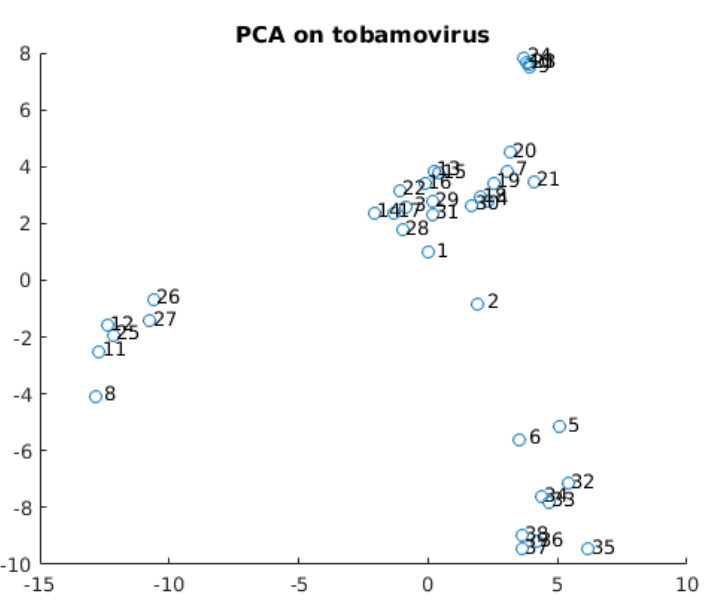
\includegraphics[width=1.0\textwidth]{./images/PCA.png}
  	\caption{Standard PCA}
  	\label{T1}
\end{figure}

\begin{figure}
	\centering
  	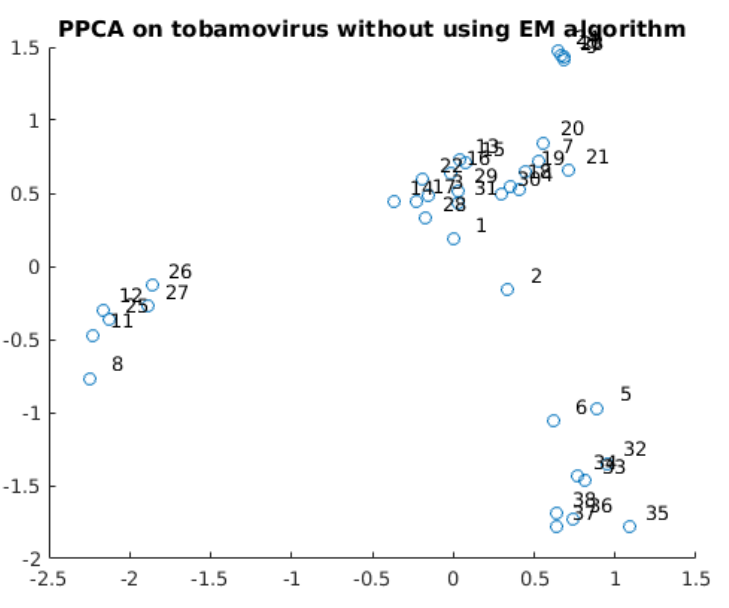
\includegraphics[width=0.7\textwidth]{./images/PPCA.png}
  	\caption{PPCA using closed form formula}
  	\label{T2}
\end{figure}

\begin{figure}
	\centering
  	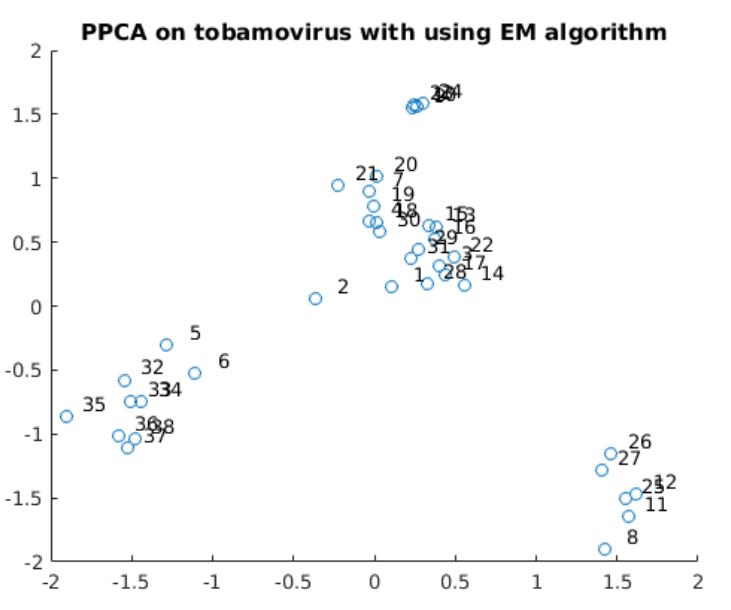
\includegraphics[width=0.7\textwidth]{./images/PPCAEM.png}
  	\caption{PPCA using EM algorithm}
  	\label{T3}
\end{figure}

\begin{figure}
	\centering
  	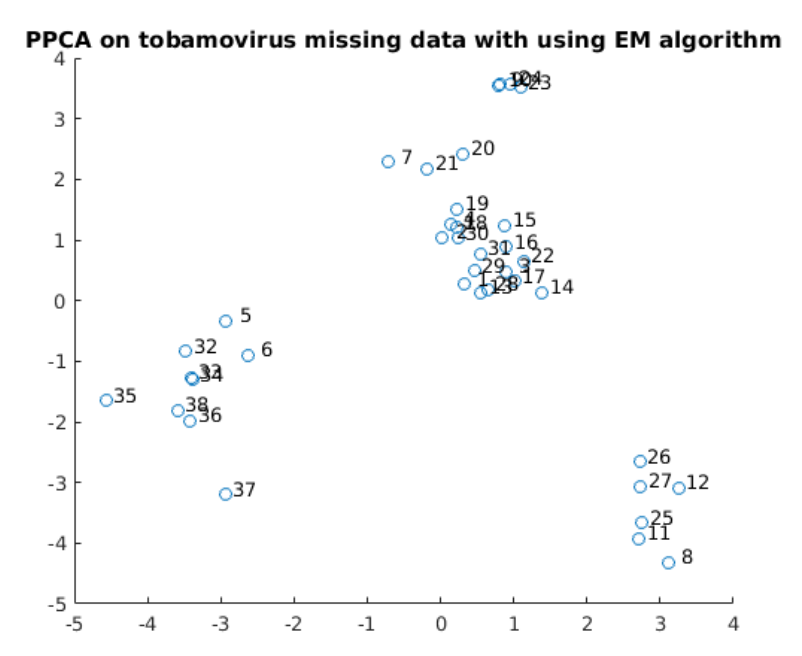
\includegraphics[width=0.7\textwidth]{./images/PPCAEMMiss.png}
  	\caption{PPCA projection with 20\% missing data using EM}
  	\label{T4}
\end{figure}

\begin{figure}
\centering
  	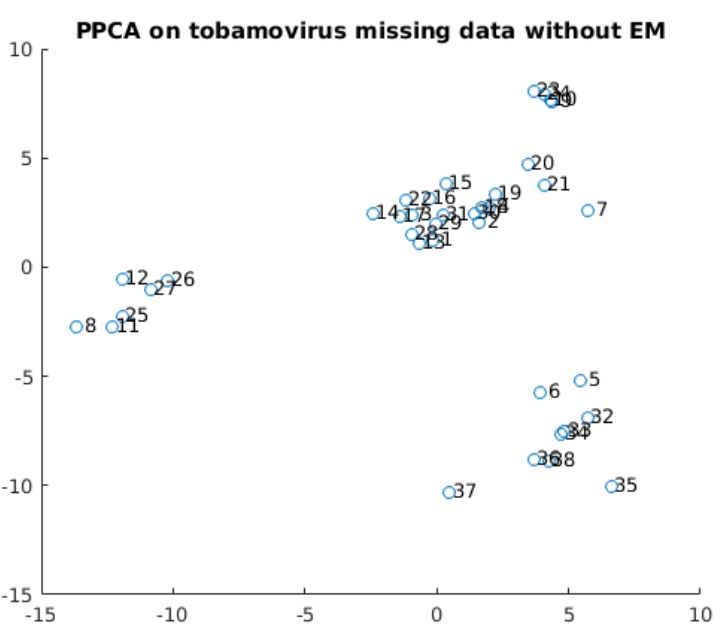
\includegraphics[width=0.7\textwidth]{./images/PCAMiss.png}
  	\caption{PCA projection with 20\% missing data}
  	\label{T5}
\end{figure}

\newpage

\section{MNIST Data}

MNIST data contains $28\times 28$ images. Each images contains a handwritten digit. The task is predition of the digits. The experiment design outlines in the last chapter is followed. \\\\
The plot \ref{T6} shows how the accuracy increases rapidly at start but then becomes static. The latent dimension $k=133$ is a good choice as it has highest accuracy in the region plotted and also the increase becomes very less after that point.\\

\begin{figure}
\centering
  	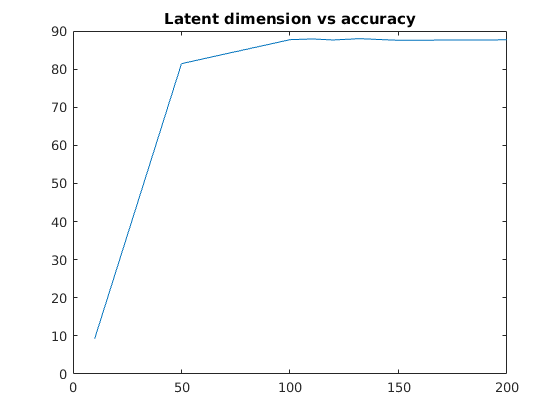
\includegraphics[width=0.8\textwidth]{./images/accuracy.png}
  	\caption{Accuracy vs latent dimension for MNIST}
  	\label{T6}
\end{figure}
The experiments that follow have $k = 133$ fixed. Following is the table showing accuracy of PPCA with missing values and comparision with other variants PCA for handling missing data. 

\newpage

\begin{table}
\begin{center}
\begin{tabular}{ |p{3cm}|p{3cm}|p{3cm}|p{3cm}|  }
 \hline
 Missing Data \% & Accuracy for PPCA with EM & Accuracy for PCA based on Factor Model & Accuracy for PCA based on $\mu$ for missing value\\
 \hline
 \hline
 	0 & 88.01 & 87.97 & 87.97\\
 	1 & 88.25 & 88.27 & 88.40\\ 
	5 & 89.62 & 91.19 & 90.30\\ 
	20 & 92.74 & 93.08 & 93.01\\
	40 & 92.44 & 71.71 & 93.05\\
	60 & 83.49 & 2.81 & 91.44\\
	80 & - & - & 86.31\\
	90 & - & - & 78.08\\
	99 & - & - & 42.94\\
 \hline
\end{tabular}
\end{center}
\caption{Accuracy for Missing data}
\label{Tb1}
\end{table}
	
From table \ref{Tb1}, we can find following observations
\begin{enumerate}
\item The accuracy increase with increase in missing data till a certain fraction. After a threshold the accuracy drops. 
\item The accuracy of PCA handling missing data based on factor model drops significantly (Column 2). The possible explanation for this is that the number of unknowns in the minimization problem $\mathbf{||y-Wx-\mu||}$ becomes large as $x$ is latent and $y$ also has missing data. So the system of equations gives poor estimates of the missing data.
\item PCA based on missing data filled by $\mu$ components show the best acuracy for missing data. A possible explanation is that a large part of data is a background image and digits occupy only lesser fraction. So larger number of missing data are estimated correclty using mean which would be towards background pixel side.
\end{enumerate}

\section{USPS Dataset}
USPS also contains handwritten digit images. The experiment outlined for MNIST is performd again for USPS. For each experiment data is randomly divided into 7 : 3 ratio for training and testing. From figure \ref{T7}, it can be seen tha $k = 100$ is an ideal choice for the latent dimension. Further experiments keep $k=100$. We can also see similar behaviour of this data set as the MNIST. Table \ref{Tb2} also contain the accuracy on conplete data as last column as the data partitioning is random.

\begin{figure}
\centering
  	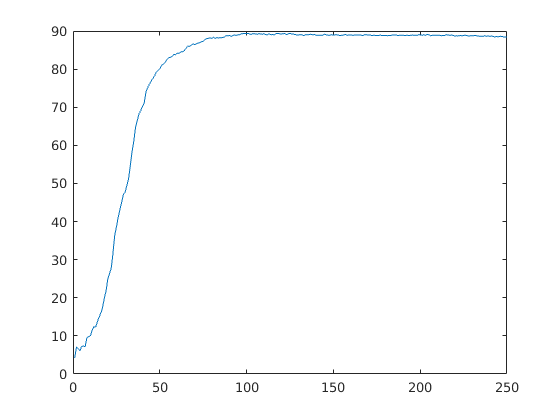
\includegraphics[width=0.8\textwidth]{./images/accuracyUSPS.png}
  	\caption{Accuracy vs latent dimension for USPS}
  	\label{T7}
\end{figure}

\begin{table}
\begin{center}
\begin{tabular}{ |p{3cm}|p{3cm}|p{3cm}|p{3cm}|p{3cm}|  }
 \hline
 Missing Data \% &Accuracy for PPCA with EM & Accuracy for PCA based on Factor Model & Accuracy for PCA based on $\mu$ for missing value & Accuracy Standard PCA on complete data\\
 \hline
 \hline
 	0.5 & 89.96 & 89.57 & 90.12 & 89.42\\
 	1 & 89.93 & 89.72 & 89.84 & 88.84\\ 
	5 & 90.51 & 90.54 & 91.90 & 88.36\\ 
	10 & 91.87 & 91.60 & 93.36 & 89.39\\	
	20 & 92.30 & 92.48 & 93.87 & 90.39 \\
	40 & 83.69 & 84.63 & 91.51 & 88.30\\
	60 & 55.21 & 52.30 & 88.75 & 88.60\\
 \hline
\end{tabular}
\end{center}
\caption{Accuracy for Missing data for USPS}
\label{Tb2}
\end{table}

\newpage

\section{Binary AlphaDigits Dataset}
The data is present in form of $39$ samples for each $36$ classes. Each sample is a $20\times 16$ image. Since the amount of data present is low picking up a large latent dimension is not feasible for calculating the mahalanobis distance. \\\\
From the plot \ref{T8}, it is clear that the accuracy increases till the number of latent dimension $k$ reaches the number of training sample ($k \sim 40$). After that the accuracy does not increase. This makes this dataset difficult to analyse. We donot any further prediction analysis for this dataset. 

\begin{figure}
\centering
  	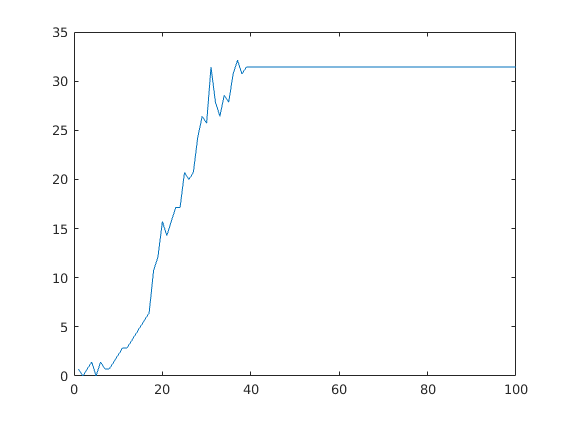
\includegraphics[width=0.8\textwidth]{./images/accuracyAlpha.png}
  	\caption{Accuracy vs latent dimension for Alpha digits}
  	\label{T8}
\end{figure}



\chapter{Conclusion}
In this work, we see how principal component analysis model can be viewed as a maximum likelihood procedure based on a probability density model of the observed data. We also see links to PPCA to factor analysis and subtle difference between the two, as well as the underlying assumption for PPCA. An EM algorithm was discussed for PPCA which iteratively maximized the likelihood of the data.\\\\
The main aim of this work was understanding PPCA and its application on real world dataset. We apply PPCA to the case of missing data and compare its performance with different version of PCA made to handle missing data. In the \emph{Results} chapter we see how PPCA is capable of handling missing data along with providing a reasonable model for interpretation of the results. But we found out that for the datasets which we covered PCA with missing data replaced by mean of non-missing data gives best performance. This leads us to conclude that for cases where data is not generated using mixtures of gaussian, the sophistication of PPCA is only to provide a probabilistic touch to the classical version of PCA.\\
The importance for EM algorithm of PPCA is more when the data has an inherent mixture model distribution. In such cases, PCA cannot trivially handle it. But PPCA could easily incorporate it into the model and handle such cases.	
\newpage

\begin{thebibliography}{1}
%Dolor
\bibitem{PPCA} 
	Tipping, Michael E., and Christopher M. Bishop. "Probabilistic principal component analysis." Journal of the Royal Statistical Society: Series B (Statistical Methodology) 61.3 (1999): 611-622.
	
\bibitem{SPCA}
Roweis, Sam. "EM algorithms for PCA and SPCA." Advances in neural information processing systems (1998): 626-632.

\bibitem{tutorial}
Chen, Haifeng. "Principal component analysis with missing data and outliers." \url{http://www.cmlab.csie.ntu.edu.tw/~cyy/learning/papers/PCA_Tutorial.pdf} (2002).
		
\bibitem{MNIST}
LeCun, Yann, Corinna Cortes, and Christopher JC Burges. "The MNIST database of handwritten digits." (1998).	
		
\bibitem{Factor}		
Whittle, Peter. "On principal components and least square methods of factor analysis." Scandinavian Actuarial Journal 1952.3-4 (1952): 223-239.	

\bibitem{PCA}
Hotelling, Harold. "Analysis of a complex of statistical variables into principal components." Journal of educational psychology 24.6 (1933): 417.	
		
\end{thebibliography}


\end{document}